\documentclass[11pt]{beamer}
%\usepackage[orientation=landscape,size=custom,width=16,height=9,scale=0.5,debug]{beamerposter} 

\usepackage[utf8]{inputenc}
\usepackage[T1]{fontenc}
\usepackage{babel}
\usepackage{lmodern}
%\usefonttheme{serif}

%\usepackage[default, osfigures]{opensans}
\usepackage[sfdefault]{FiraSans}

\usepackage{amsmath}
\usepackage{amsfonts}
\usepackage{amssymb}
\usepackage{graphicx}
\usetheme{Boadilla}
\usepackage{hyperref}
\usepackage{multirow}
\usepackage{longtable}
\usepackage{tabularx}
\usepackage{rotating}
\usepackage{siunitx}
\usepackage{multirow}
\usepackage{array} 
\usepackage{booktabs}
\newcommand{\head}[1]{\textnormal{\textbf{#1}}}

\usepackage{tikz}
\usetikzlibrary{spy}

\setbeamertemplate{section in toc}[circle]
\setbeamertemplate{itemize items}[default]
\setbeamertemplate{itemize subitem}[square]
\setbeamertemplate{itemize subsubitem}[circle]
\setbeamertemplate{itemize mini template}[ball]

\setbeamertemplate{enumerate items}[circle]
\setbeamertemplate{enumerate subitem}[square]
\setbeamertemplate{enumerate subsubitem}[circle]
\setbeamertemplate{enumerate mini template}[ball]


\renewcommand{\baselinestretch}{1.3}
\setbeamersize{text margin left=0.5cm}
\setbeamersize{text margin right=0.5cm}


%\setbeamertemplate{footline}[frame number]







\setbeamertemplate{footline}
{%
	\begin{beamercolorbox}{section in head/foot}
		\vskip-1.7pt \insertnavigation {\paperwidth } \vskip-3.1pt   





	\end{beamercolorbox}%
}
\setbeamertemplate{navigation symbols}{}

%\setbeamercolor{block title}{fg = white, bg = gray}
%\setbeamercolor{block body}{fg = black, bs = blue!30}
\usepackage[most]{tcolorbox}

\setbeamertemplate{blocks}[rounded][shadow=false] % use rounded blocks with standard beamer shadow


\begin{document}
	\author[Nith Kosal]{Nith Kosal}
	\title[Presentation Title]{\bfseries Data Visualization}
	\subtitle{\bfseries A Practical Introduction}
	\titlegraphic{\includegraphics[width=0.2\linewidth]{Figure/Logo}}

	
	\institute{Future Forum}
	\date[\today]{2021 YRP Seminar, May 18, 2021}
	%\subject{}
	%\setbeamercovered{transparent}
	%\setbeamertemplate{navigation symbols}{}

	\begin{frame}[plain]
		\maketitle
		
	\end{frame}
%------------------------------------------------------------------%
% Page number set from 1 into page 2
	\addtobeamertemplate{navigation symbols}{}{     
		\usebeamerfont{footline}%
		\insertframenumber/\inserttotalframenumber }
	\setcounter{framenumber}{0}
%------------------------------------------------------------------%	
\section{Goals}
	\begin{frame}

	\frametitle{\bfseries Goal of Today's Seminar}
	
	\begin{itemize}
		\item Know the types of graphs we should avoid 
		\item Learn about RStudio IDE (integrated development environment) 
		\item Data visualization in R
		\item Data import and transformation
		\item Data export 
		\item Discussion about your questions or any concerns about R or datasets   
	\end{itemize}

\textbf{Remember:} It will not work in a flow and structure, because we practice in the real example as a researcher have a dataset and applied it for a specific research study.
\end{frame}
%------------------------------------------------------------------%
\section{R Sources}
	
	\begin{frame}

	\frametitle{\bfseries Seminar Materials}
	
	\begin{itemize}
		\item You can code, data and slide from my repository at GitHub: \url{https://github.com/nithkosal/DataVisualization}
		\item Intermediate level: R for Data Science by Hadley Wickham and Garrett Grolemund. Available online:
		\url{https://r4ds.had.co.nz/}
		\item Advanced R by Hadley Wickham. Also available here:
		\url{https://adv-r.hadley.nz/}
		\item R Blog: \url{https://www.r-bloggers.com/}
		\item Ask questions or share your knowledge about programming:
		\url{https://stackoverflow.com/questions/tagged/r}
	\end{itemize}
	
	
\end{frame}
%------------------------------------------------------------------%

	\begin{frame}

		\frametitle{\bfseries The Thing to know when you work with data}
		
		\begin{figure}
			\centering
			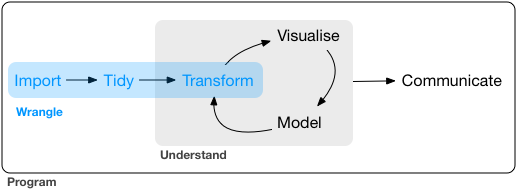
\includegraphics[width=0.8\linewidth]{Figure/data-science}
			\\ 
			\footnotesize Source: Grolemund and Wickham (2016)
			\label{fig:data-science}
		\end{figure}

	\begin{itemize}
		\item Tidying your data means storing it in a consistent form that matches the semantics of the dataset with the way it is stored.
		
		\item Together, tidying and transforming, we called \textit{wrangling}

		
		
	\end{itemize}
	\end{frame}
%------------------------------------------------------------------%
	
	\begin{frame}
		\section[]{}
		\frametitle{\bfseries What does data visualization mean?}
		
		\begin{itemize}
			\item A reporting tool: the representation of information in the form of a chart, diagram, picture, etc.
			\item It is a part of \textit{hypothesis generation} or \textit{data exploration}. 
			\begin{itemize}
				\item A precise mathematical model to generate falsifiable predictions.
				\item Only use an observation once to confirm a hypothesis.
			\end{itemize}
		\item Modelling is an important part of the exploratory process.
		\end{itemize}

	\end{frame}
%------------------------------------------------------------------%
\section{Definition}

\begin{frame}

	\frametitle{\bfseries Now, We Look at Some Data Visualizations}
	\begin{figure}
		\vspace{-.5em}
		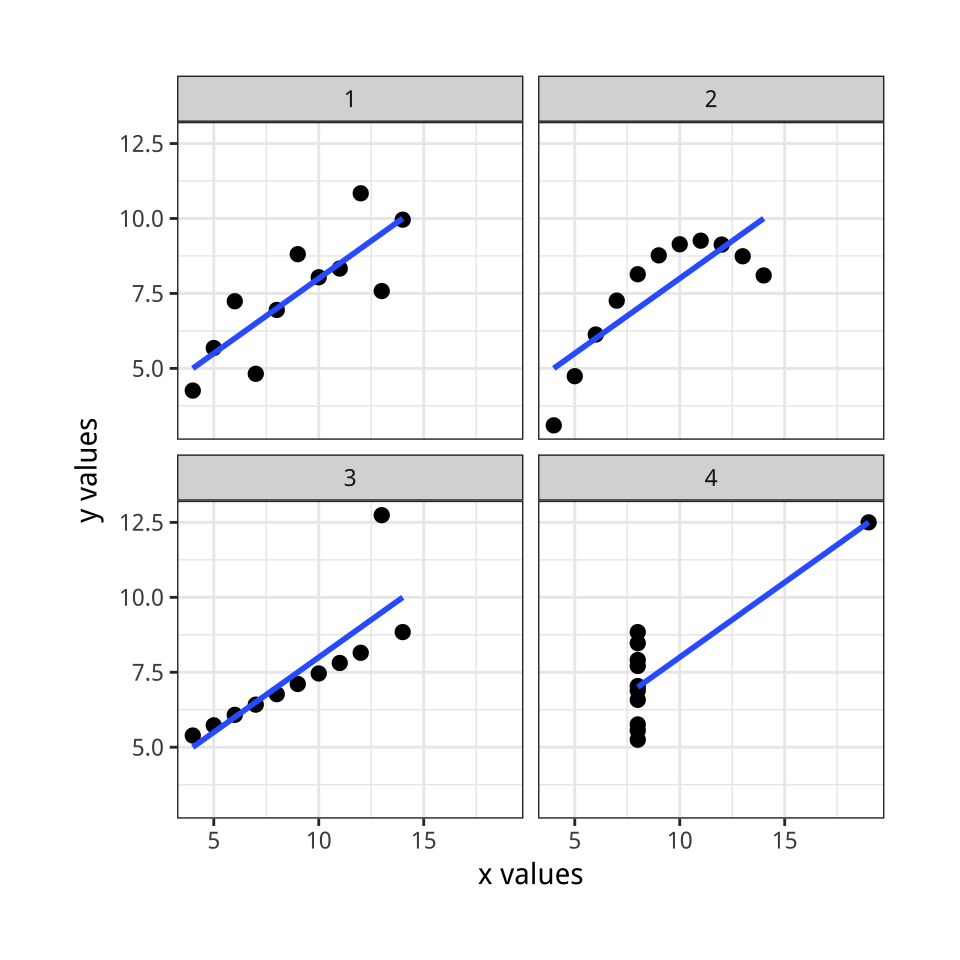
\includegraphics[width=0.5\linewidth]{Figure/anscombe-1}
		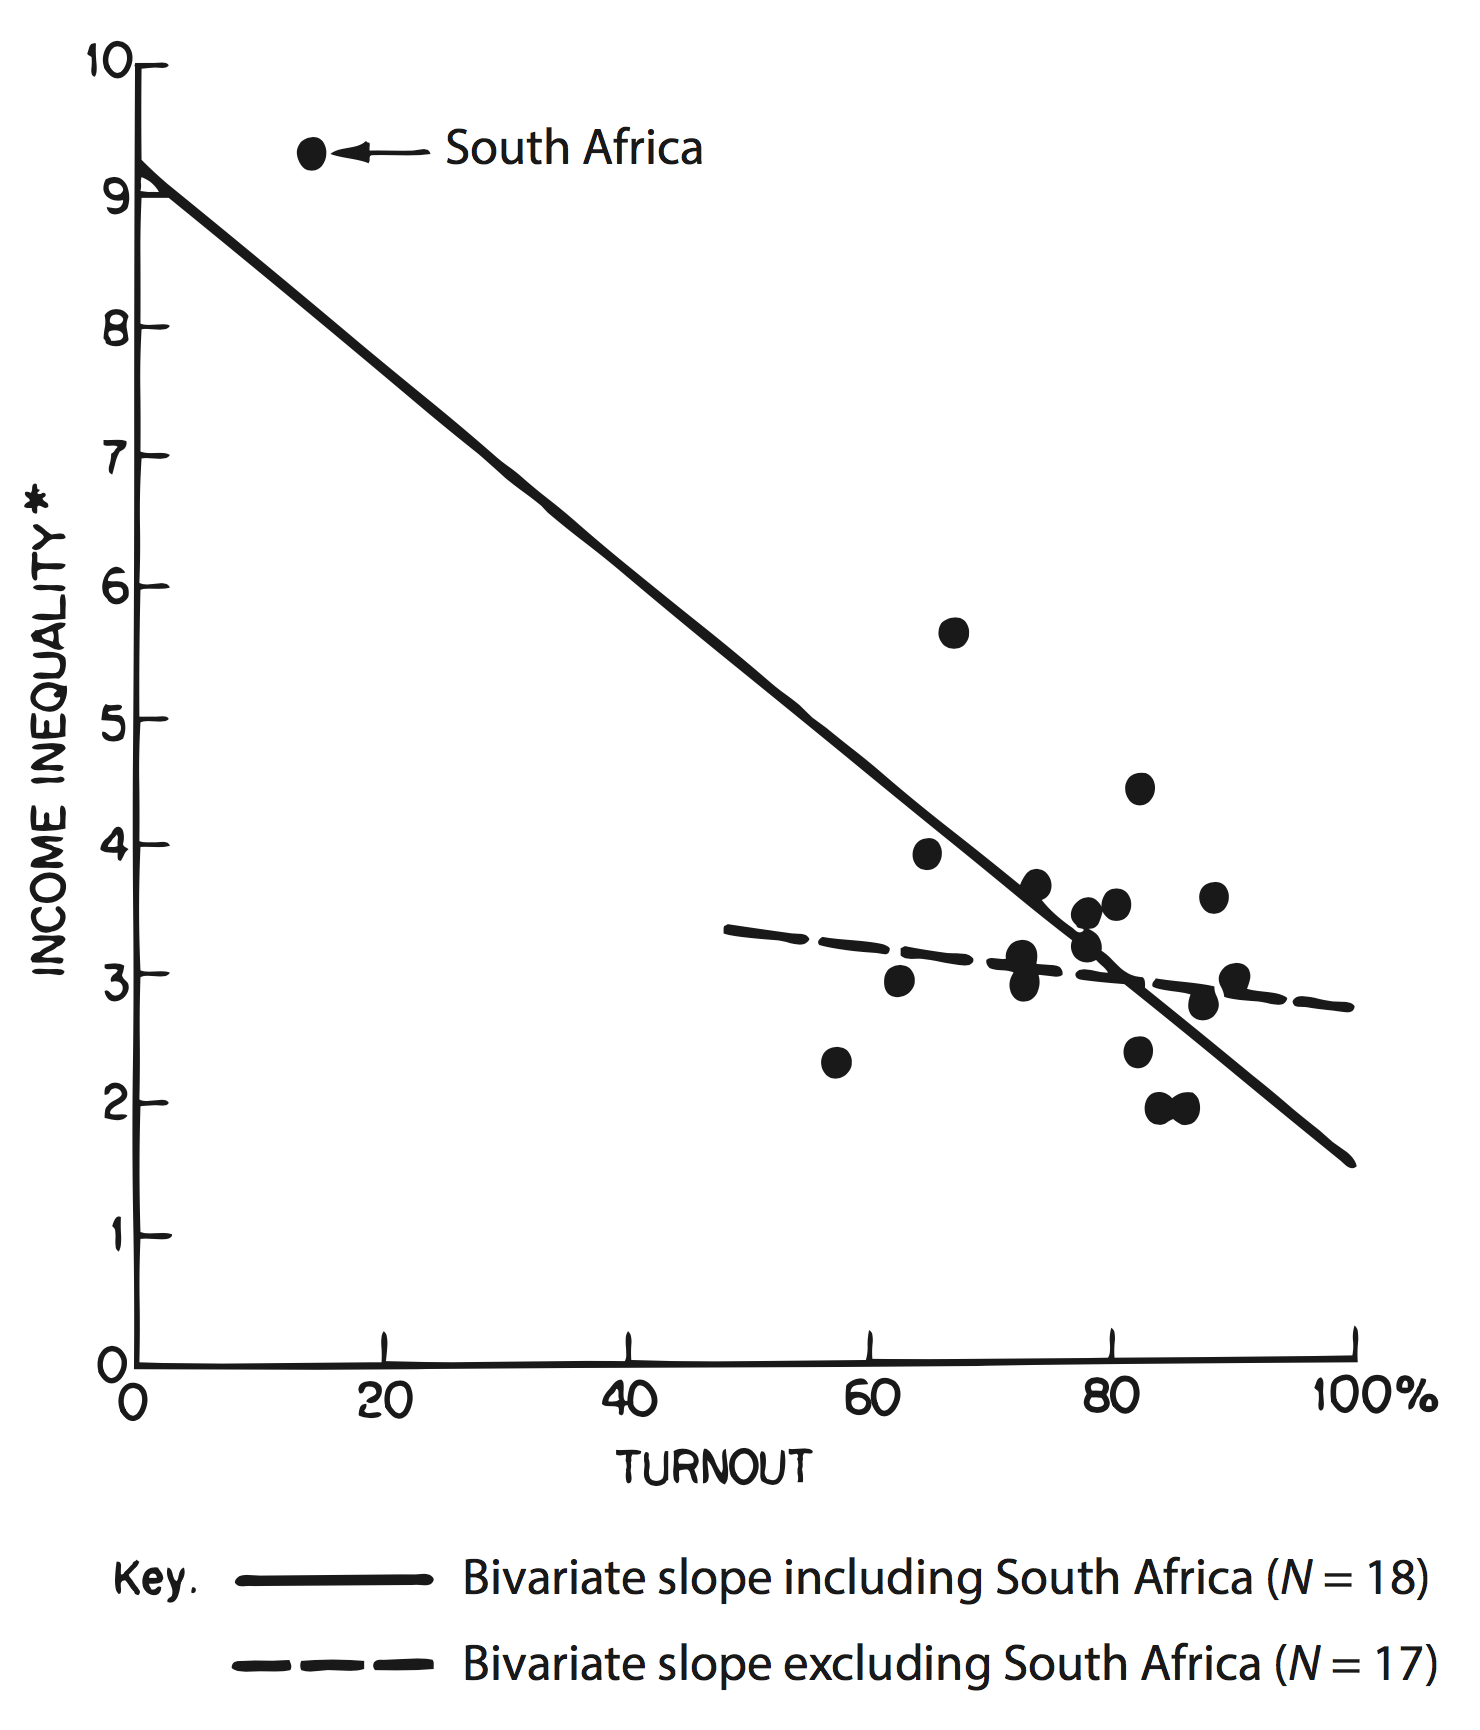
\includegraphics[width=0.4\linewidth]{Figure/jackman-outlier}
		\\
		\tiny{Source: Chatterjee and Firat (2007), Jackman (1980)}
		\label{fig:anscombe-1}
	\end{figure}
	\begin{itemize}
		\footnotesize{
		\item Scatterplots are the workhorse of data visualization in social science.
		\item A scatterplot shows the relationship between two quantities, such as height and weight, age and income, or time and unemployment. }
	\end{itemize}
\end{frame}
%------------------------------------------------------------------%
\section{Good Figures}
\begin{frame}
	
	\frametitle{\bfseries}
			\vspace{-1em}
			
			\begin{tabular}{p{2.6cm}p{8.6cm}}
				\footnotesize{
					Within each panel, the correlation between the \texttt{x} and \texttt{y} variables is set to be \texttt{0.6}, a pretty good degree of association. But the actual distribution of points is created by a different process in each case.} & 
				\begin{figure}
					\vspace{-1.7em}
					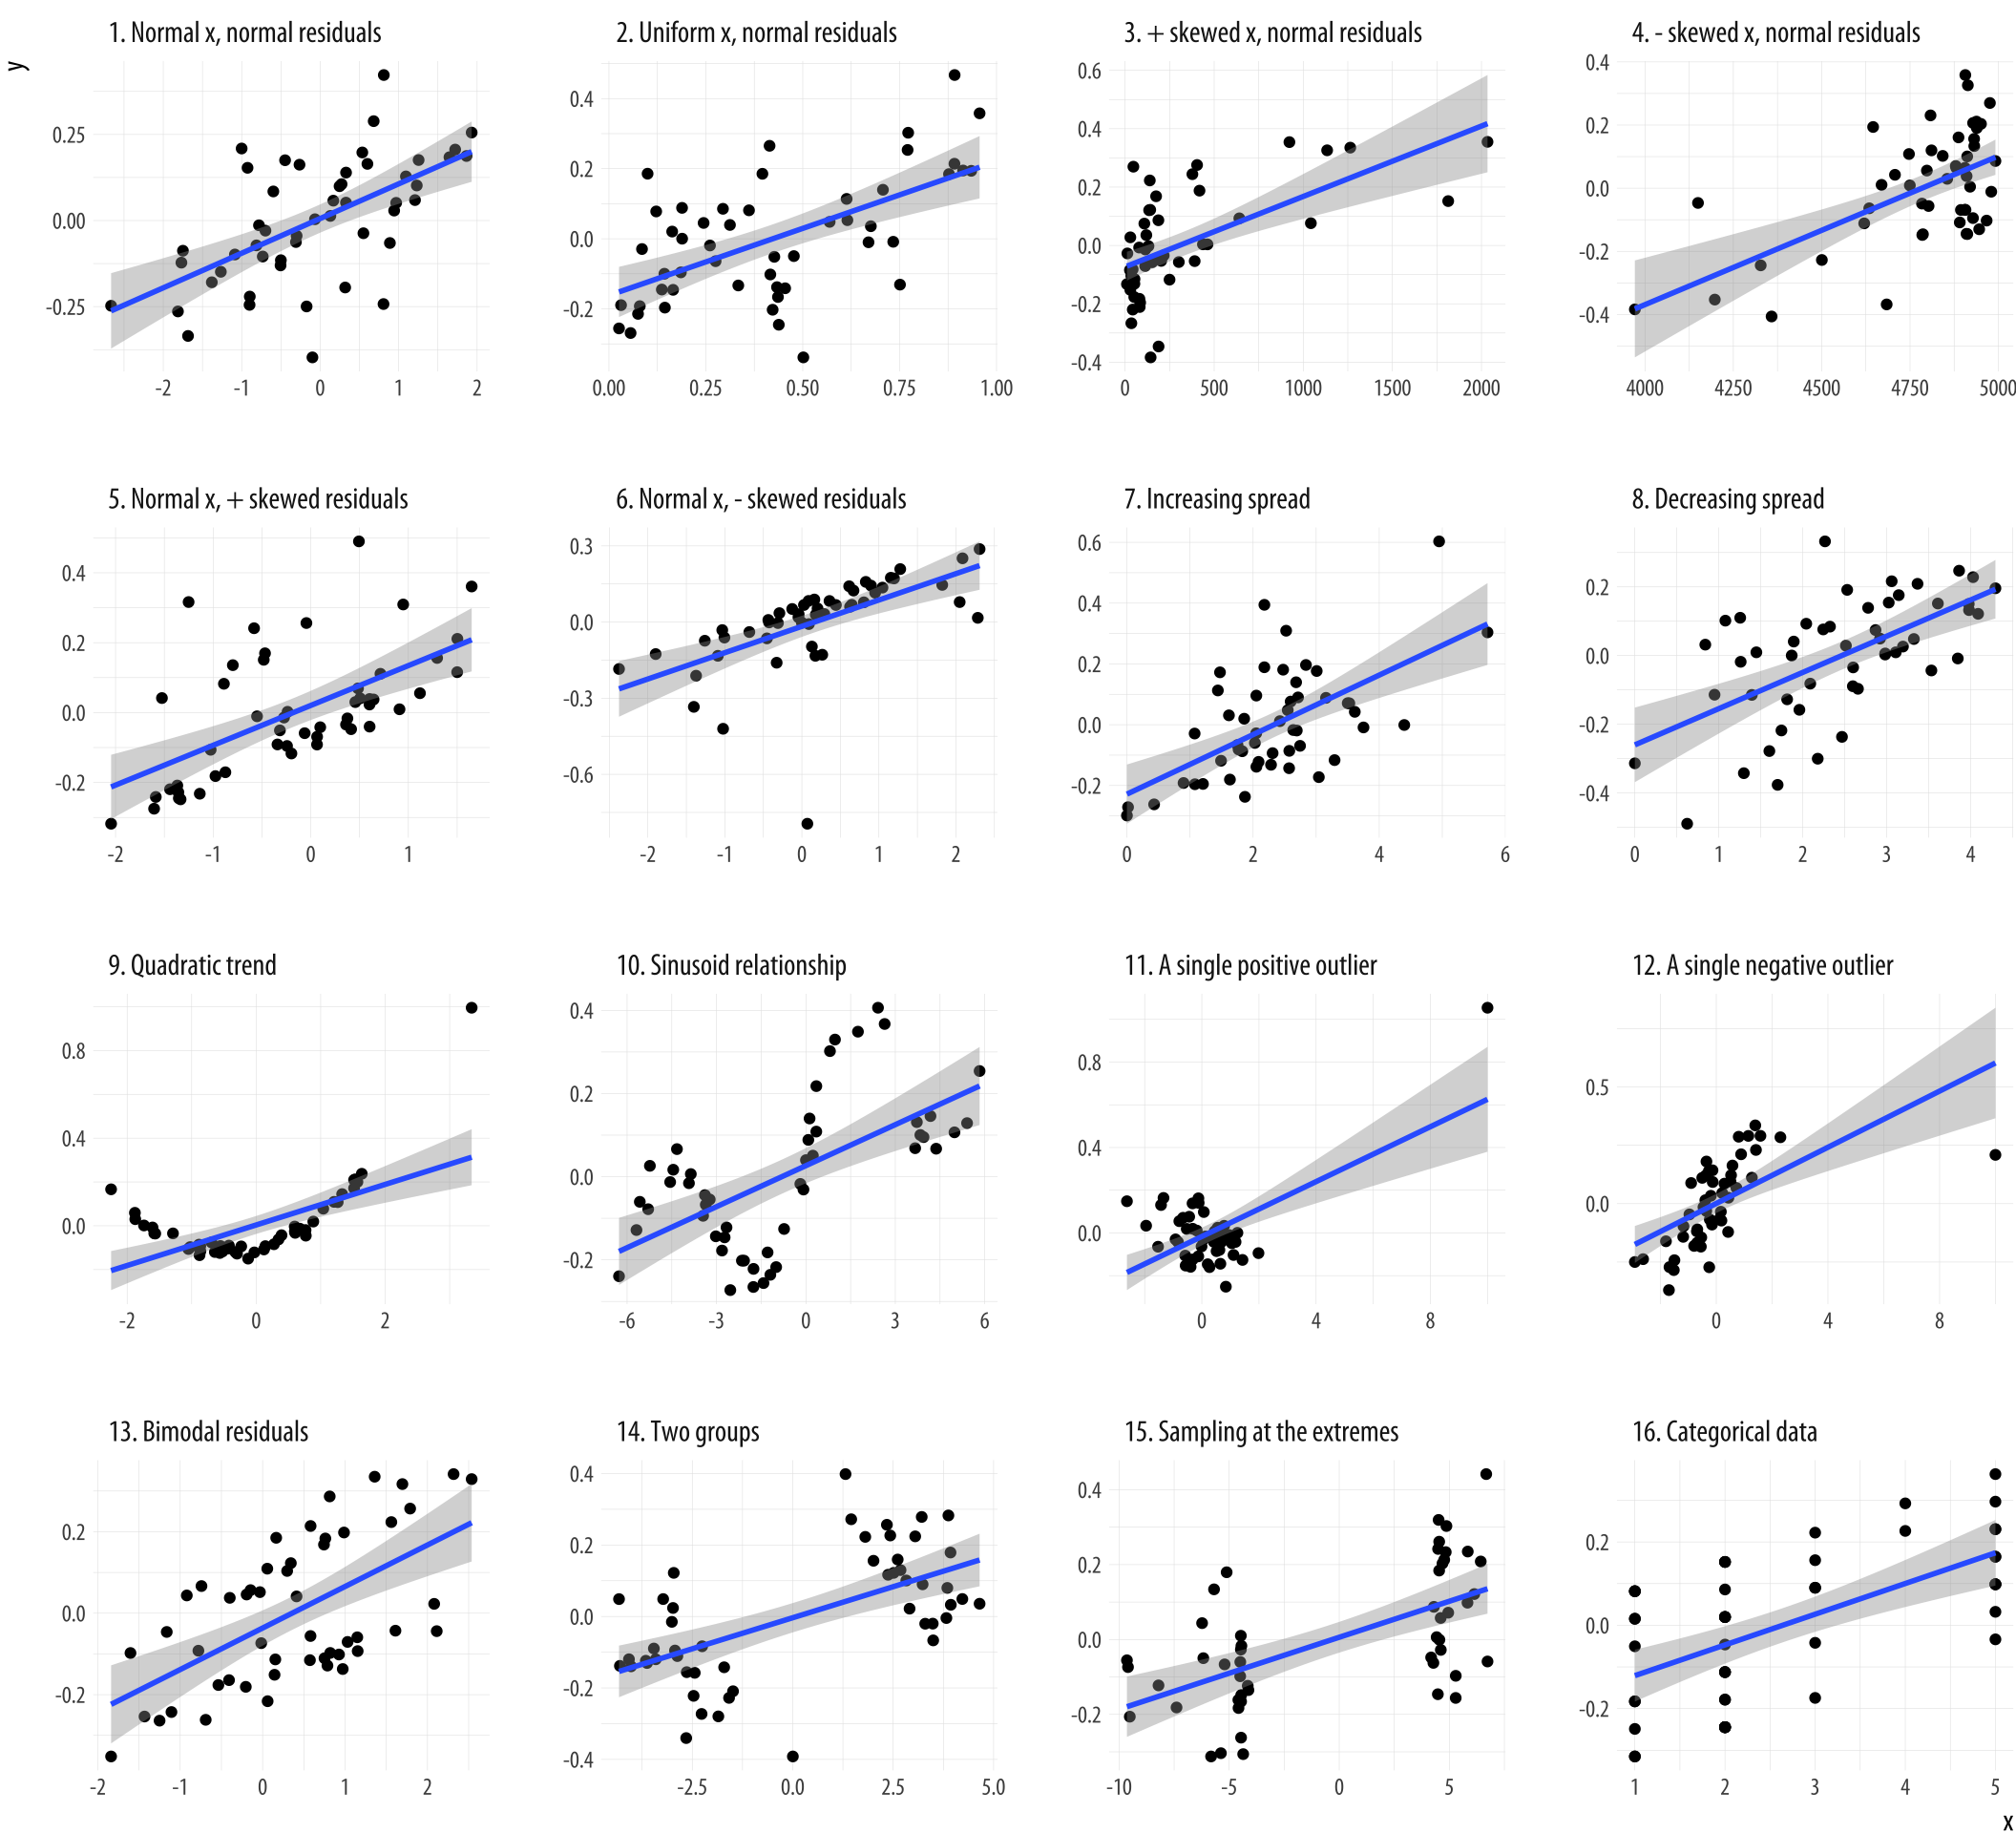
\includegraphics[width=1\linewidth]{Figure/correlations-1}\raggedleft
					\label{fig:correlations-1}
					\\
					\tiny{Source: Jan Vanhove (2016)}
				\end{figure}
				
			\end{tabular}
			
\end{frame}
%------------------------------------------------------------------%
\section{Bad Figures}
\begin{frame}
	
	\frametitle{\bfseries}
	\vspace{-1em}
	\centering{
			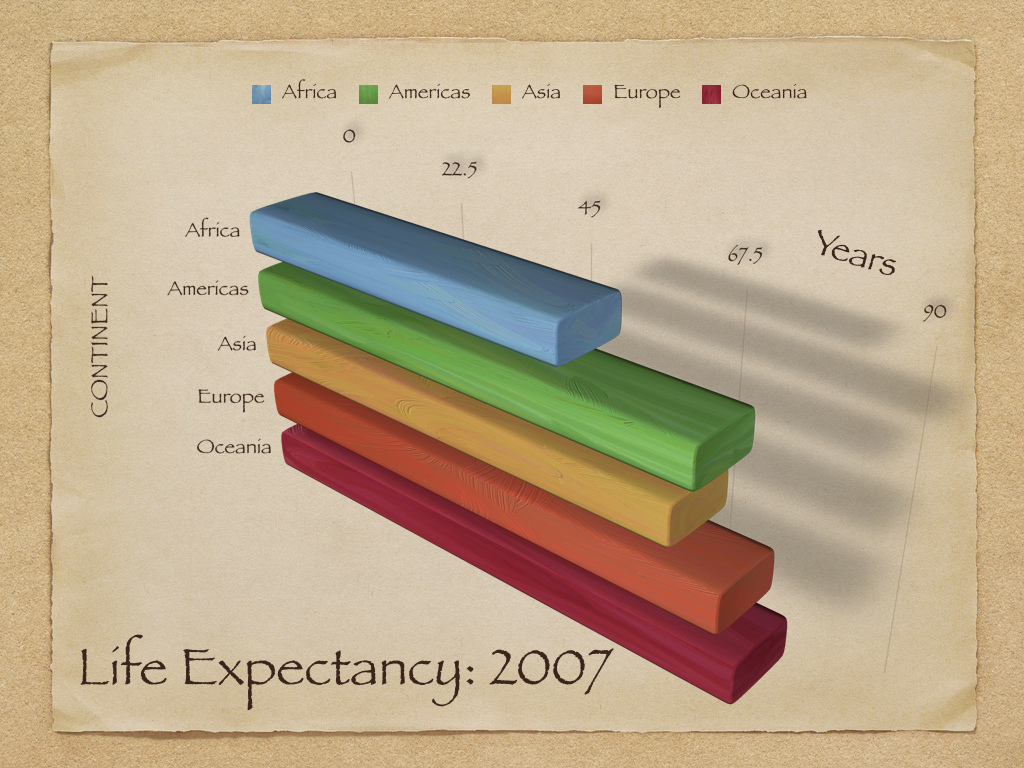
\includegraphics[width=.8\linewidth]{Figure/chartjunk-life-expectancy}
			\\ \vspace{-1em}
			\tiny{Source: Kieran Healy (2018)}}\\
		The bars are hard to read and compare.
\end{frame}
%------------------------------------------------------------------%

\begin{frame}
	
	\frametitle{\bfseries}
	\begin{figure}
		\vspace{-1em}
		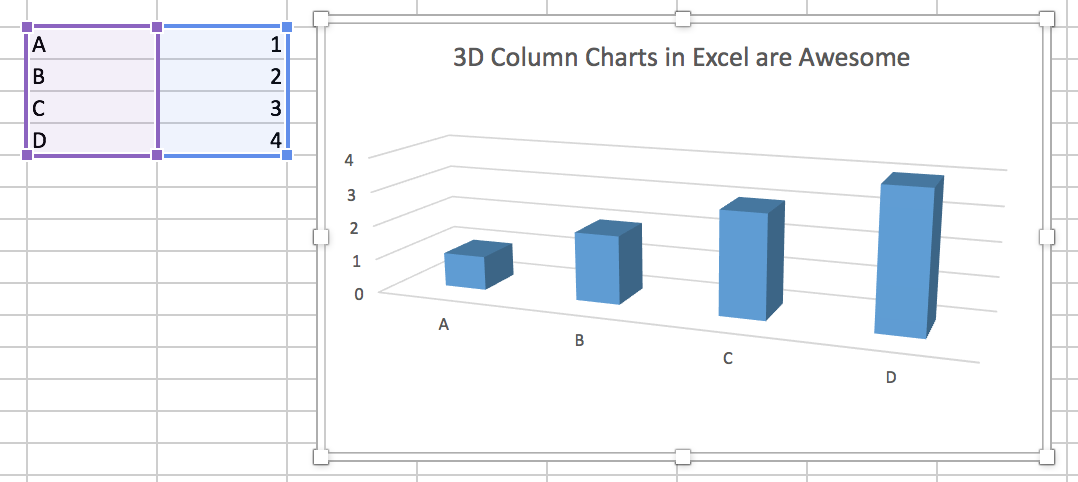
\includegraphics[width=0.9\linewidth]{Figure/excel-3d-column-chart-values}
		\\
		\tiny{A 3-D Column Chart created in Microsoft Excel}
	\end{figure}
	\begin{itemize}
		\vspace{-1em}
		\footnotesize{
			\item Charts like this are common in business presentations and popular journalism, and are also seen in academic journal articles. Here we seek to avoid too much junk by using Excel’s default settings.
			 
		 }
	\end{itemize}
\end{frame}
%------------------------------------------------------------------%

\begin{frame}
	
	\frametitle{\bfseries}
	\vspace{-1em}
	{\centering
		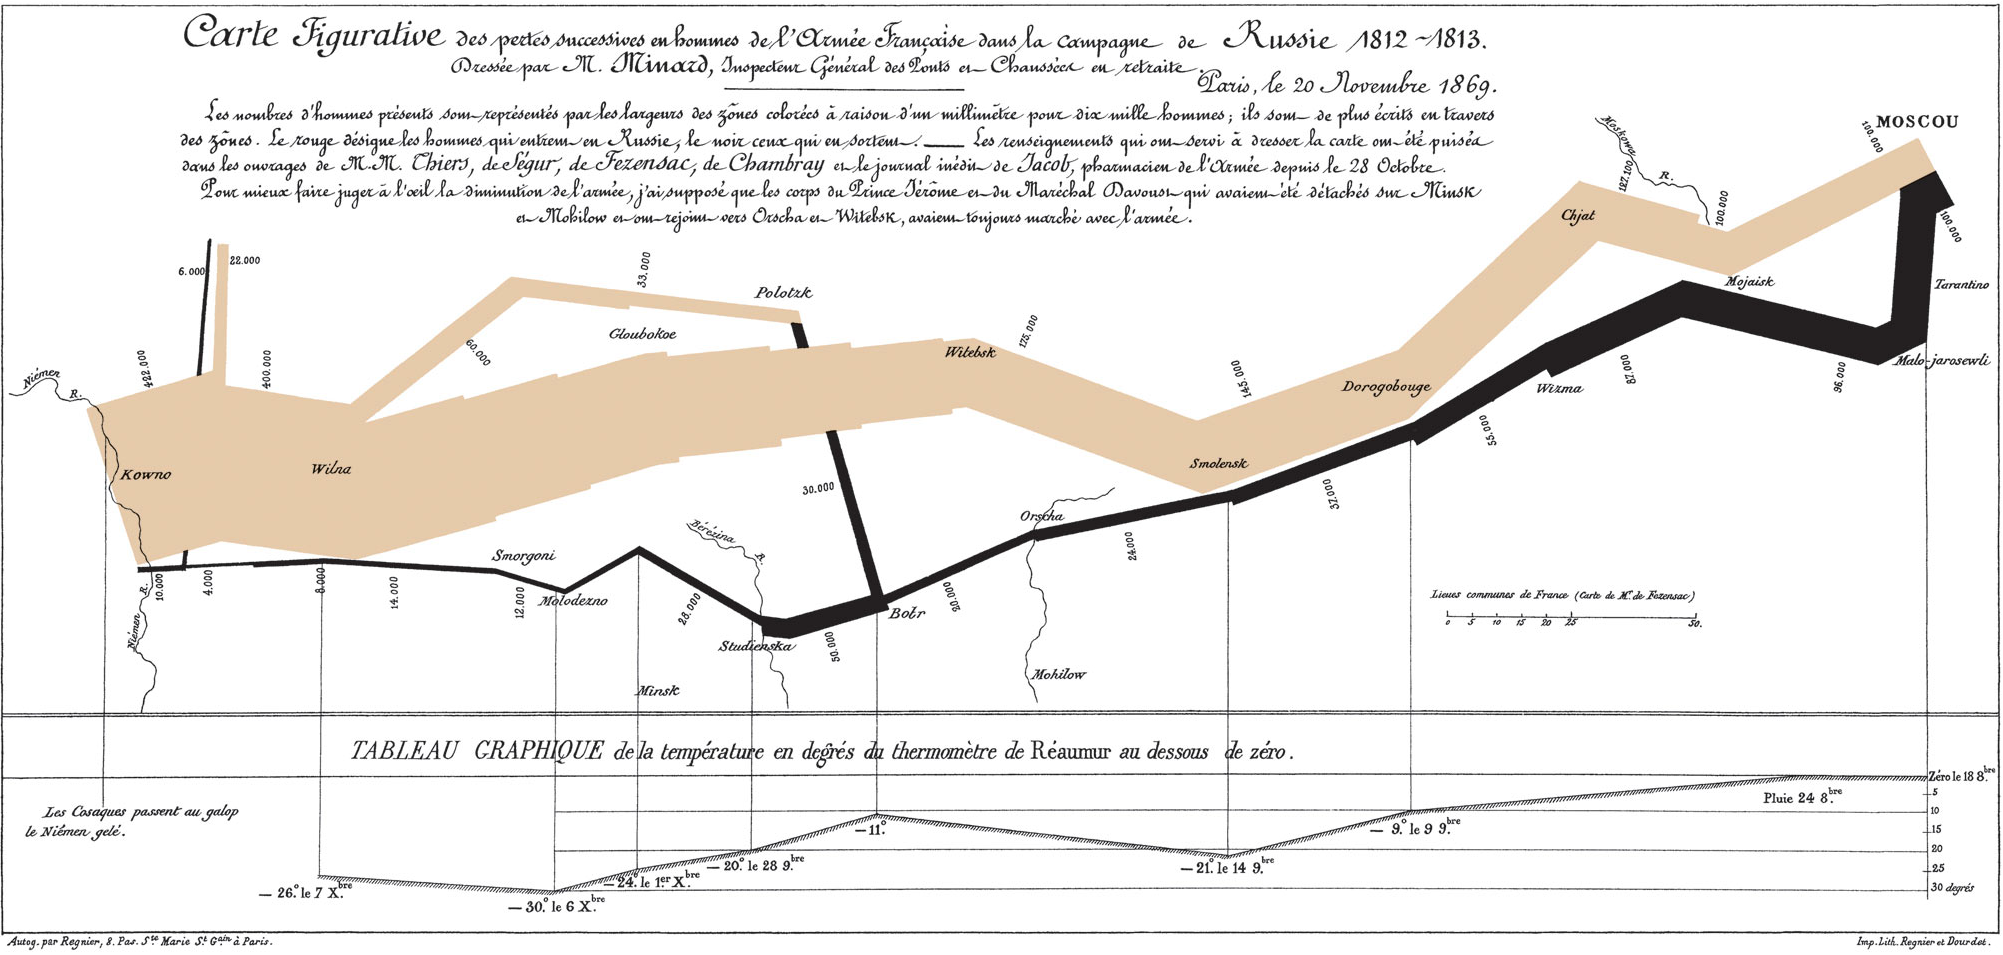
\includegraphics[width=1\linewidth]{Figure/minard}
		\\ 	\vspace{-1em}
		\tiny{Source: Charles Joseph Minard --- Minard’s visualization of Napoleon’s retreat from Moscow.}}\\
	\footnotesize {Edward Tufte's comment: ``\textit{Graphical excellence is the well-designed presentation of interesting data—a matter of substance, of statistics, and of design, it consists of complex ideas communicated with clarity, precision, and efficiency.}''}
\end{frame}
%------------------------------------------------------------------%


\begin{frame}
	
	\frametitle{\bfseries}
	\begin{figure}
		\vspace{-.5em}
		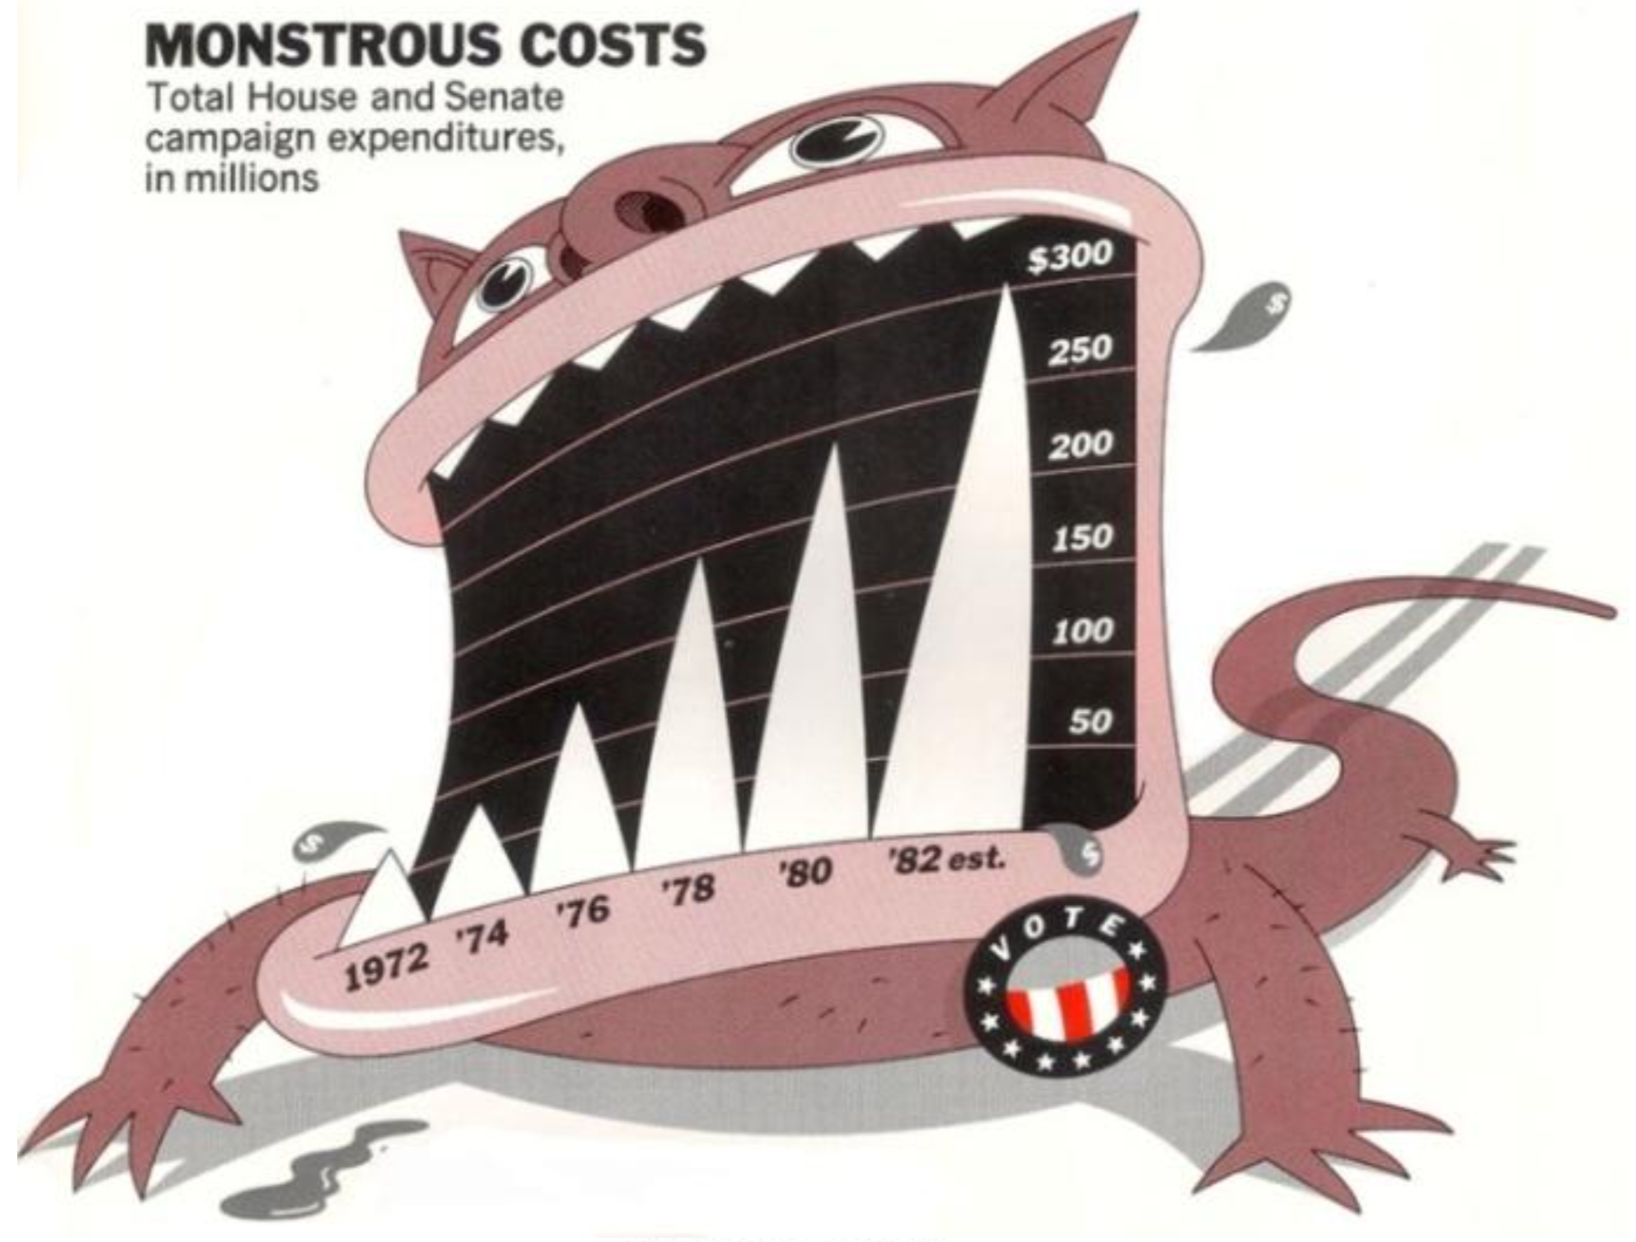
\includegraphics[width=0.6\linewidth]{Figure/holmes-monstrous-only}

		\\
		\tiny{Source: `Monstrous Costs’ by Nigel Holmes}
		\label{fig:anscombe-1}
	\end{figure}
	\begin{itemize}
		\footnotesize{
			\item Viewers do not find them more easily interpretable, but they do remember them more easily and also seem to find them more enjoyable to look at.
			\item Borkin et al. (2013) found that ``\textit{Infographic}'' style graphs were more memorable than more standard statistical visualizations. }
	\end{itemize}
\end{frame}
%------------------------------------------------------------------%

\begin{frame}
	
	\frametitle{\bfseries}
	\begin{figure}
		\vspace{-1em}
		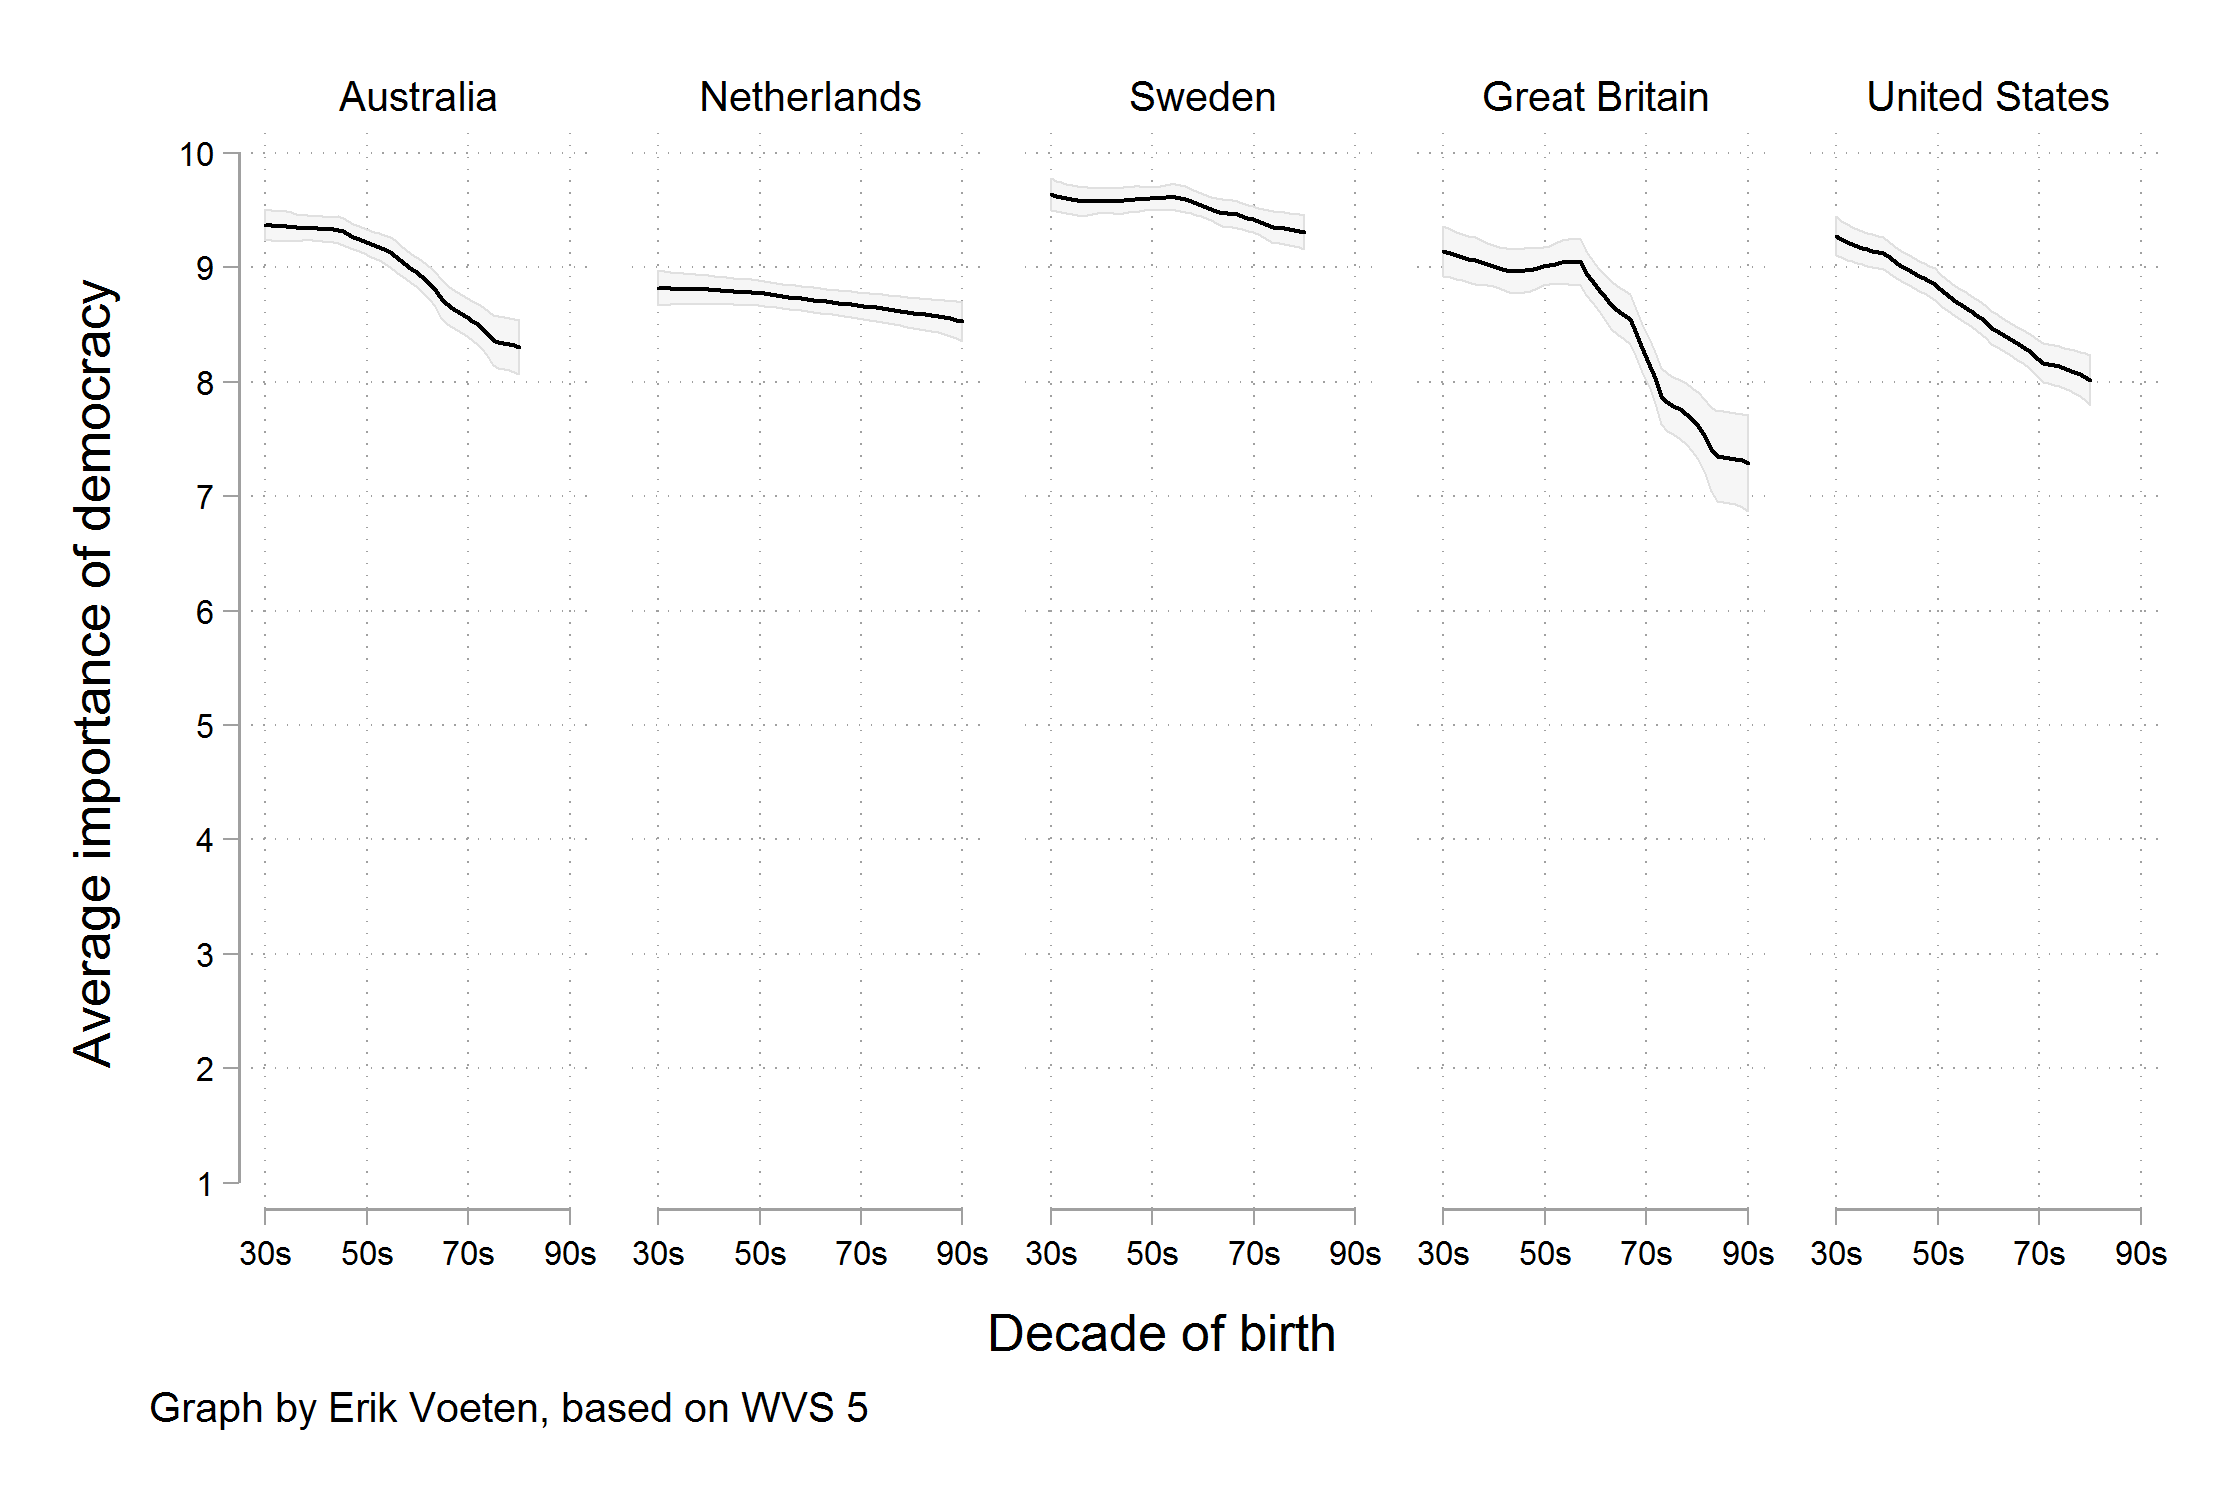
\includegraphics[width=1\linewidth]{Figure/democracy-voeten-version-2}
	\end{figure}
	\begin{itemize}
		
	\end{itemize}
\end{frame}
%------------------------------------------------------------------%
\begin{frame}
	
	\frametitle{\bfseries}
	\begin{figure}
		\vspace{-.5em}
		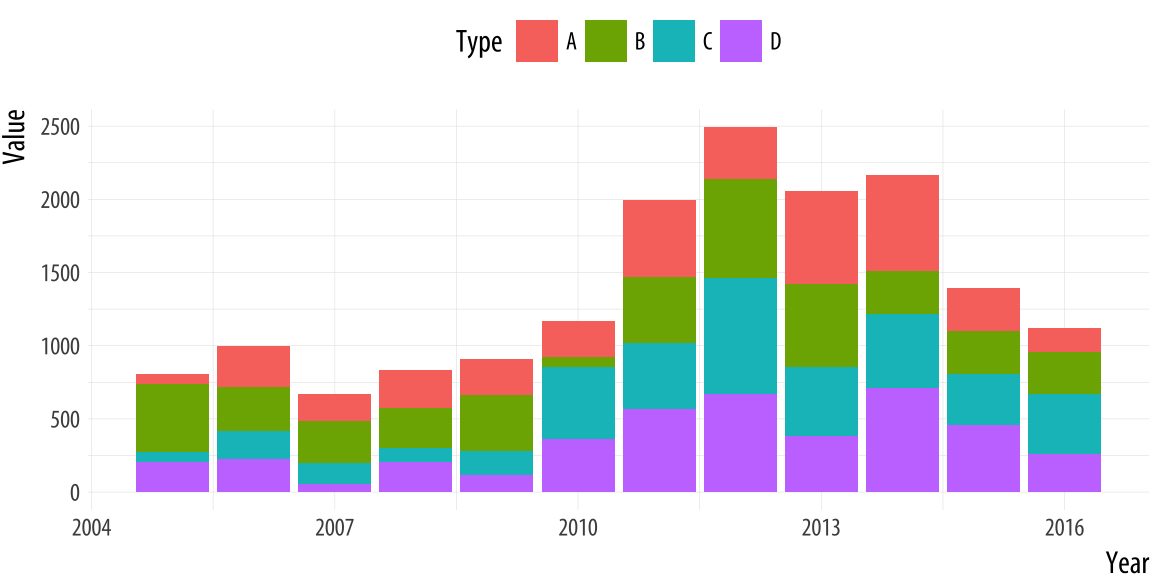
\includegraphics[width=0.8\linewidth]{Figure/preception-data-1}
		
		\\
		\tiny{A junk-free plot that remains hard to interpret}
		\label{fig:anscombe-1}
	\end{figure}
	\begin{itemize}
		\footnotesize{
			\item The bars show the total value, with subdivisions by the relative contribution of different categories to each year’s observation.
			\item Charts like this are common when showing the absolute contribution of various products to total sales over time, or the number of different groups of people in a changing population.
		}
	\end{itemize}
\end{frame}
%------------------------------------------------------------------%

\begin{frame}
	
	\frametitle{\bfseries}
	\begin{figure}
		\vspace{-.5em}
		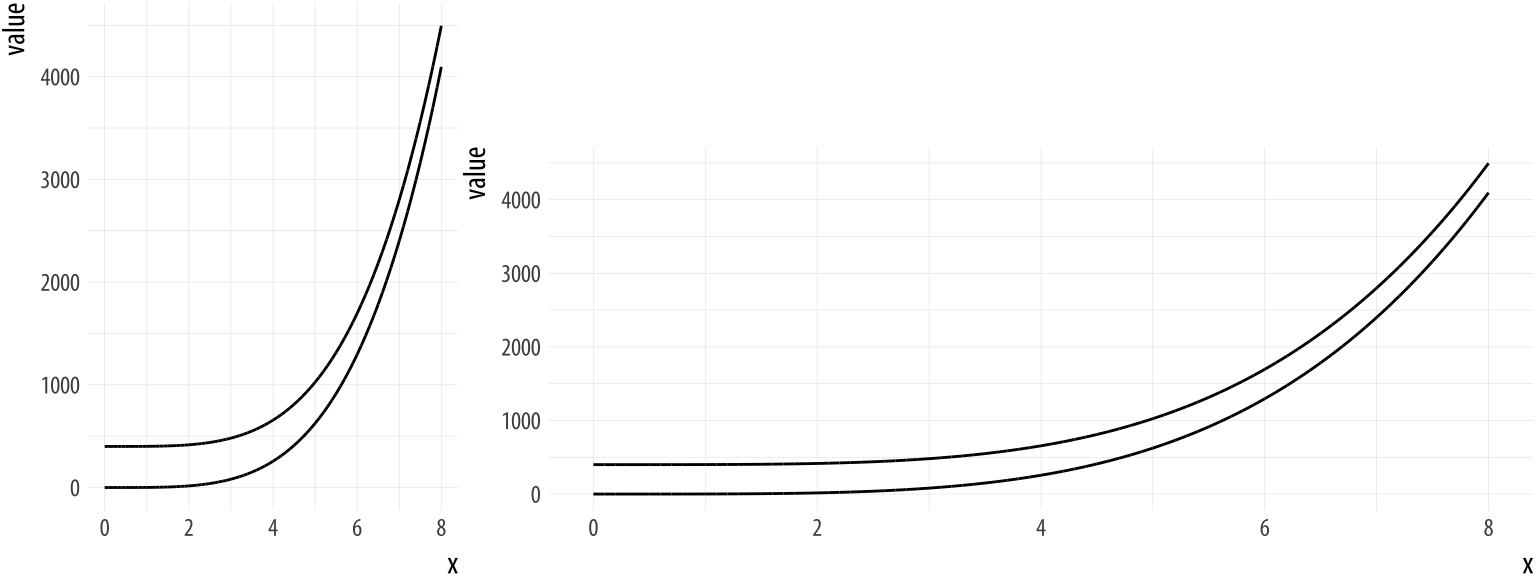
\includegraphics[width=0.9\linewidth]{Figure/perception-curves-1}
		
		\\
		\tiny{Source: An example by William S. Cleveland}
		\label{fig:anscombe-1}
	\end{figure}
	\begin{itemize}
		\footnotesize{
			\item In the left-side panel, the lines appear at first glance to be converging as the value of x increases.
			\item The data plotted in each panel are the same, however. The apparent convergence in the left panel is just a result of the aspect ratio of the figure. 
		}
	\end{itemize}

\end{frame}
%------------------------------------------------------------------%

\begin{frame}
	
	\frametitle{\bfseries}
	\begin{block}{In Short}
	These problems are not easily solved by the application of good taste, or by following a general rule to maximize the data-to-ink ratio, even though that is a good rule to follow. Instead, we need to know a little more about the role of perception in the interpretation of graphs. 
	\end{block}

\end{frame}
%------------------------------------------------------------------%

\section{Variables}
\begin{frame}

	\frametitle{\bfseries Variable Types in the Statistical Software}
	
	\begin{enumerate}
		\item \texttt{int} stands for intergers
		\item \texttt{dbl} stands for doubles, or we call real numbers
		\item \texttt{chr} stands for character vectors, and strings
		\item \texttt{dttm} stands for date-times (a date + a time)
	\end{enumerate}

At the same time, there are three other common types of variables
	\begin{enumerate}
		\item \texttt{lgl} stands for logical, vectors that contain only \texttt{TRUE} or \texttt{FALSE}
		\item \texttt{fctr} stands for factors, which R uses to represent categorical variables with fixed possible values.
		\item \texttt{date} stands for dates.
	\end{enumerate}
	
\end{frame}
%------------------------------------------------------------------%

\section{Practice}
	\begin{frame}
	\frametitle{\bfseries}
		\begin{beamercolorbox}{title}
		\begin{center}
			\bfseries \huge Let us go practice!
		\end{center}	
	\end{beamercolorbox}
	
	\end{frame}
%------------------------------------------------------------------%


\end{document}